\documentclass[14pt,a4paper]{extarticle}
\usepackage{graphicx}
\usepackage{caption} 
\usepackage{hyperref}
\usepackage[T1]{fontenc}
\usepackage[utf8x]{inputenc}
\usepackage{pdfpages}
\usepackage{libertine}
\usepackage{listings}
\usepackage{xcolor}
\usepackage{enumitem}
\usepackage{fullpage}
\usepackage{ulem}
\usepackage{cancel}

\renewcommand{\thesection}{\arabic{section}}
\renewcommand{\familydefault}{\sfdefault}



\definecolor{stringgreen}{rgb}{0.0, 0.5, 0.0}

\lstset{
  literate={ö}{{\"o}}1
           {ä}{{\"a}}1
           {ü}{{\"u}}1
           {Ö}{{\"O}}1
}

\lstdefinestyle{fish}{
	basicstyle=\small\ttfamily\color{black},
    keywordstyle=\color{blue},
	stringstyle=\medium\ttfamily\color{green},
    numberstyle=\tiny\color{gray},
    showstringspaces=false,
    tabsize=4,
	frame=single,
    breaklines=true,
    morekeywords={sudo,if,then,else,elif,fi,for,do,done,while,until,in},
}

\lstdefinestyle{json}{
	basicstyle=\small\ttfamily\color{black},
    showstringspaces=false,
    tabsize=2,
    breaklines=true,
}

\lstdefinestyle{sql}{
	basicstyle=\small\ttfamily\color{black},
    keywordstyle=\color{blue},
	stringstyle=\color{stringgreen},
    numberstyle=\tiny\color{gray},
    showstringspaces=false,
	frame=single,
    tabsize=4,
    breaklines=true,
	language=SQL
}

\colorlet{punct}{red!60!black}
\definecolor{delim}{RGB}{20,105,176}
\colorlet{numb}{magenta!60!black}

\hypersetup{
    colorlinks=true,
    linkcolor=blue,
    filecolor=blue,      
    urlcolor=blue,
    pdfborder={0 0 0},
    linktocpage      
}

\begin{document}
	\begin{titlepage}
		\centering
		{\scshape\LARGE Big Data \par}
		\vspace{2.5cm}
		{\huge\bfseries Graph Databases}
		\vfill
		{\normalsize von\par}
		{\normalsize Benjamin Ellmer (\textsc{S2210455012}) \par}
		\vspace{1cm}
		
\includegraphics[width=0.3\textheight]{images/logo.pdf} \par
		\vspace{1cm}
		{\large Mobile Computing Master \par}
		{\large FH Hagenberg \par}
		\vfill
		{\large \today\par}
	\end{titlepage}

	\section*{Installation}
	\noindent \textbf{Start Neo4j}
	\begin{lstlisting}[style=fish]
git clone https://github.com/Digital-Media/neo4j.git
docker compose -f neo4j/docker-compose.yml up -d
	\end{lstlisting}

	\noindent \textbf{Start Postgres}
	\begin{lstlisting}[style=fish]
docker run --name postgres-big-data-ex4 -e POSTGRES_PASSWORD=geheim -d postgres:14
	\end{lstlisting}

	\section*{Step 1 - Translation}
	\noindent \textbf{Connect to postgres container}
	\begin{lstlisting}[style=sql]
docker exec -it postgres-big-data-ex4 psql -U postgres
	\end{lstlisting}

	\noindent \textbf{Drop, create and select schema:}
	\begin{lstlisting}[style=sql]
DROP SCHEMA IF EXISTS graph_demos CASCADE;
CREATE SCHEMA IF NOT EXISTS graph_demos;
SET search_path TO graph_demos;
	\end{lstlisting}

	\noindent \textbf{Create folks table:}
	\begin{lstlisting}[style=sql]
CREATE TABLE IF NOT EXISTS folks (
	id bigint NOT NULL,
	name varchar(100) NOT NULL,
	father bigint NULL,
	mother bigint NULL,
	PRIMARY KEY (id),
	CONSTRAINT father_fk FOREIGN KEY (father) REFERENCES folks(id),
	CONSTRAINT mother_fk FOREIGN KEY (mother) REFERENCES folks(id)
);
	\end{lstlisting}

	\newpage
	
	\noindent \textbf{Insert folks:}
	\begin{lstlisting}[style=sql]
INSERT INTO folks (id, name, father, mother) VALUES
(100, 'Alex', 20, 30),
(20, 'Dad', 10, null),
(30, 'Mom', null, null),
(10, 'Grandpa Bill', null, null),
(98, 'Sister Amy', 20, 30);
	\end{lstlisting}

	\noindent \textbf{Create vertices table:}
	\begin{lstlisting}[style=sql]
CREATE TABLE vertices (
	vertex_id bigint NOT NULL,
	alias varchar (255),
	label varchar (255),
	name varchar (255),
	type varchar (255),
	properties jsonb,
	PRIMARY KEY (vertex_id)
);
	\end{lstlisting}

	\noindent \textbf{Insert vertices:}
	\begin{lstlisting}[style=sql]
INSERT INTO vertices (vertex_id, alias, label, name, type) VALUES
(1, 'NAmerica', 'Location', 'North America', 'continent'),
(2, 'Europe', 'Location', 'Europe', 'continent'),
(3, 'USA', 'Location', 'United States', 'country'),
(4, 'UK', 'Location', 'United Kingdom', 'country'),
(5, 'England', 'Location', 'England', 'country'),
(6, 'Austria', 'Location', 'Österreich', 'country'),
(7, 'Idaho', 'Location', 'Idaho', 'state'),
(8, 'London', 'Location', 'London', 'city'),
(9, 'UpperAustria', 'Location', 'Oberösterreich', 'Bundesland'),
(10, 'Waldviertel', 'Location', 'Waldviertel', 'Viertel'),
(11, 'Grein', 'Location', 'Grein', 'city'),
(12, 'Andrea', 'Person', 'Andrea', 'person'),
(13, 'Bert', 'Person', 'Bert', 'person'),
(14, 'Christian', 'Person', 'Christian', 'person');
	\end{lstlisting}

	\newpage

	\noindent \textbf{Create edges table:}
	\begin{lstlisting}[style=sql]
CREATE TABLE edges (
	edge_id bigint NOT NULL,
	tail_vertex bigint REFERENCES vertices (vertex_id),
	head_vertex bigint REFERENCES vertices (vertex_id),
	label varchar(255),
	properties jsonb,
	PRIMARY KEY (edge_id),
	CONSTRAINT tail_vertex_fk FOREIGN KEY (tail_vertex) REFERENCES vertices(vertex_id),
	CONSTRAINT head_vertex_fk FOREIGN KEY (head_vertex) REFERENCES vertices(vertex_id)
);
	\end{lstlisting}

	\noindent \textbf{Insert edges:}
	\begin{lstlisting}[style=sql]
INSERT INTO edges (edge_id, tail_vertex, head_vertex, label) VALUES
(1, 3, 1, 'within'),
(2, 4, 2, 'within'),
(3, 5, 4, 'within'),
(4, 6, 2, 'within'),
(5, 7, 3, 'within'),
(6, 8, 5, 'within'),
(7, 9, 6, 'within'),
(8, 10, 9, 'within'),
(9, 11, 10, 'within'),
(10, 12, 7, 'born_in'),
(11, 12, 8, 'lives_in'),
(12, 13, 11, 'born_in'),
(13, 13, 8, 'lives_in'),
(14, 14, 8, 'born_in'),
(15, 12, 13, 'married'),
(16, 13, 12, 'married');
	\end{lstlisting}

	\pagebreak

	\section*{Step 2}
	\noindent \textbf{Connect to neo4j container:}
	\begin{lstlisting}[style=sql]
docker exec -it neo4j cypher-shell -u neo4j -p password
	\end{lstlisting}

	\noindent \textbf{Create Folks with relationships:}
	\begin{lstlisting}[style=sql]
CREATE (alex:Folk {id: 100, name: 'Alex'})
CREATE (dad:Folk {id: 20, name: 'Dad'})
CREATE (mom:Folk {id: 30, name: 'Mom'})
CREATE (grandpa:Folk {id: 10, name: 'Grandpa Bill'})
CREATE (amy:Folk {id: 98, name: 'Sister Amy'})

CREATE (dad)-[:FATHER]->(alex)
CREATE (mom)-[:MOTHER]->(alex)

CREATE (dad)-[:FATHER]->(amy)
CREATE (mom)-[:MOTHER]->(amy)

CREATE (alex)-[:BROTHER]->(amy)
CREATE (amy)-[:SISTER]->(alex)

CREATE (grandpa)-[:FATHER]->(dad);
	\end{lstlisting}

	\begin{center}
		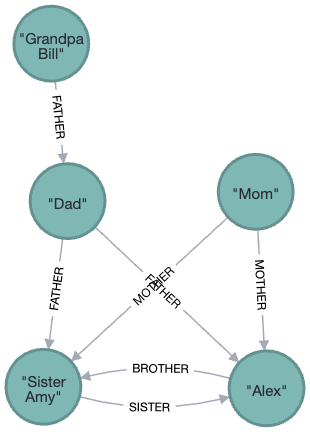
\includegraphics[height=9cm]{images/folks.png}
	\end{center}

	\pagebreak

	\noindent \textbf{Create Locations with relationships:}
	\begin{lstlisting}[style=sql]
CREATE (namerica:Location {alias: 'NAmerica', label: 'Location', name: 'North America', type: 'continent'})
CREATE (europe:Location {alias: 'Europe', label: 'Location', name: 'Europe', type: 'continent'})
CREATE (usa:Location {alias: 'USA', label: 'Location', name: 'United States', type: 'country'})
CREATE (uk:Location {alias: 'UK', label: 'Location', name: 'United Kingdom', type: 'country'})
CREATE (england:Location {alias: 'England', label: 'Location', name: 'England', type: 'country'})
CREATE (austria:Location {alias: 'Austria', label: 'Location', name: 'Österreich', type: 'country'})
CREATE (idaho:Location {alias: 'Idaho', label: 'Location', name: 'Idaho', type: 'state'})
CREATE (london:Location {alias: 'London', label: 'Location', name: 'London', type: 'city'})
CREATE (upperaustria:Location {alias: 'UpperAustria', label: 'Location', name: 'Oberösterreich', type: 'Bundesland'})
CREATE (waldviertel:Location {alias: 'Waldviertel', label: 'Location', name: 'Waldviertel', type: 'Viertel'})
CREATE (grein:Location {alias: 'Grein', label: 'Location', name: 'Grein', type: 'city'})

CREATE (usa)-[:WITHIN]->(namerica)
CREATE (uk)-[:WITHIN]->(europe)
CREATE (england)-[:WITHIN]->(uk)
CREATE (austria)-[:WITHIN]->(europe)
CREATE (idaho)-[:WITHIN]->(usa)
CREATE (london)-[:WITHIN]->(england)
CREATE (upperaustria)-[:WITHIN]->(austria)
CREATE (waldviertel)-[:WITHIN]->(upperaustria)
CREATE (grein)-[:WITHIN]->(waldviertel);
	\end{lstlisting}

	\pagebreak

	\noindent \textbf{Create Persons with relationships:}
	\begin{lstlisting}[style=sql]
MATCH (idaho:Location {alias: 'Idaho'})
MATCH (london:Location {alias: 'London'})
MATCH (grein:Location {alias: 'Grein'})

CREATE (andrea:Person {alias: 'Andrea', label: 'Person', name: 'Andrea', type: 'person'})
CREATE (bert:Person {alias: 'Bert', label: 'Person', name: 'Bert', type: 'person'})
CREATE (christian:Person {alias: 'Christian', label: 'Person', name: 'Christian', type: 'person'})

CREATE (andrea)-[:BORN_IN]->(idaho)
CREATE (andrea)-[:LIVES_IN]->(london)

CREATE (bert)-[:BORN_IN]->(grein)
CREATE (bert)-[:LIVES_IN]->(london)

CREATE (christian)-[:BORN_IN]->(london)
	
CREATE (andrea)-[:MARRIED]->(bert)
CREATE (bert)-[:MARRIED]->(andrea);
	\end{lstlisting}

	\pagebreak

	\noindent \textbf{Show the whole graph:}
	\begin{lstlisting}[style=sql]
MATCH (n) OPTIONAL MATCH (n)-[r]-() RETURN n, r;
	\end{lstlisting}
	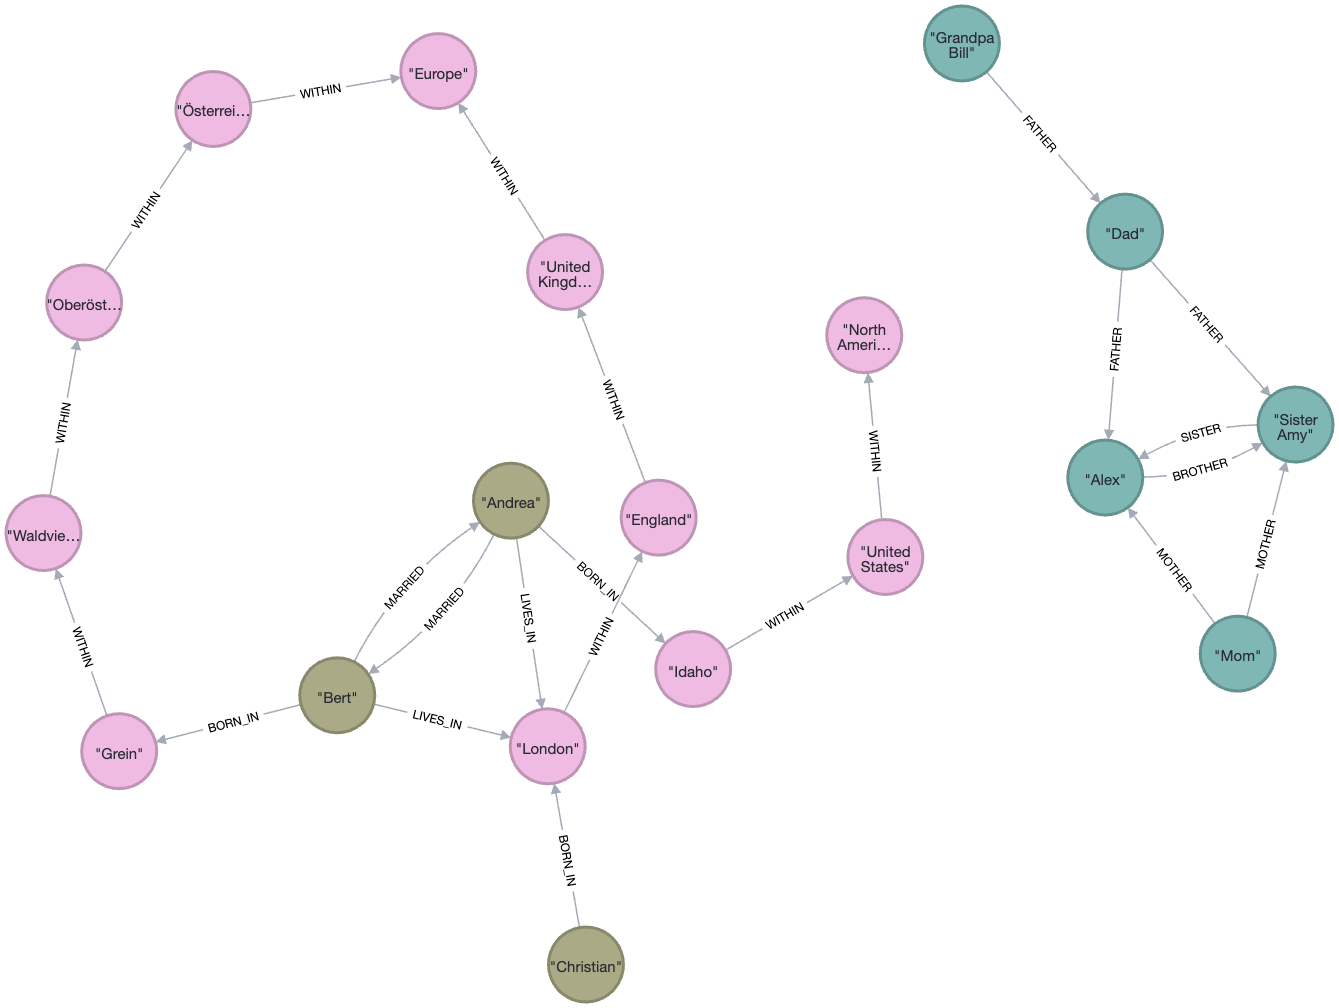
\includegraphics[width=\textwidth]{images/whole graph.png}

	\noindent \textbf{Read all :Person nodes:}
	\begin{lstlisting}[style=sql]
MATCH (p:Person) RETURN p;
	\end{lstlisting}
	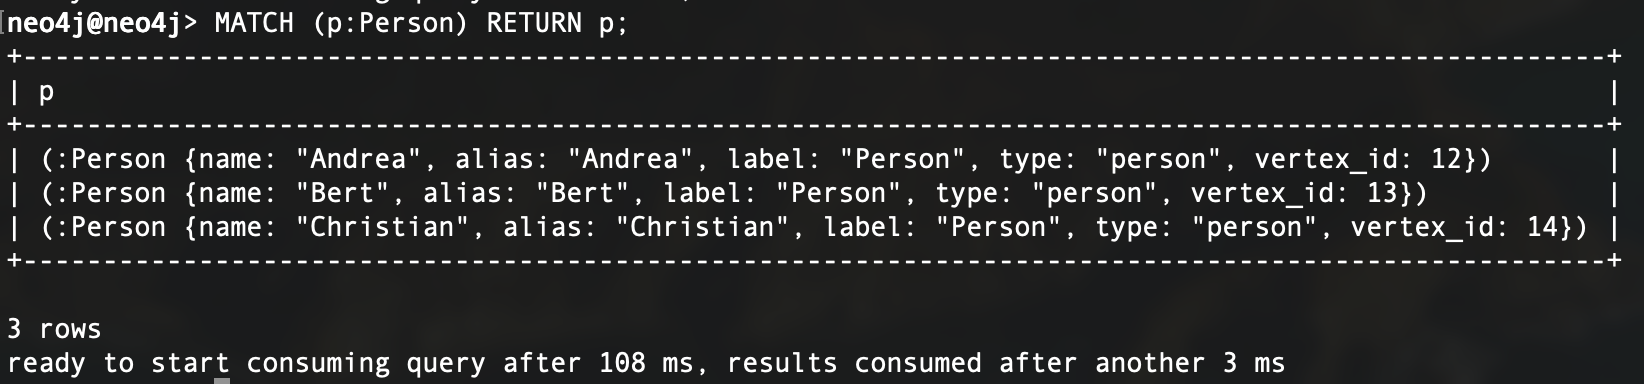
\includegraphics[width=\textwidth]{images/sc02.png}

	\pagebreak

	\noindent \textbf{Return all names of :Person nodes:}
	\begin{lstlisting}[style=sql]
MATCH (p:Person) RETURN p.name;
	\end{lstlisting}
	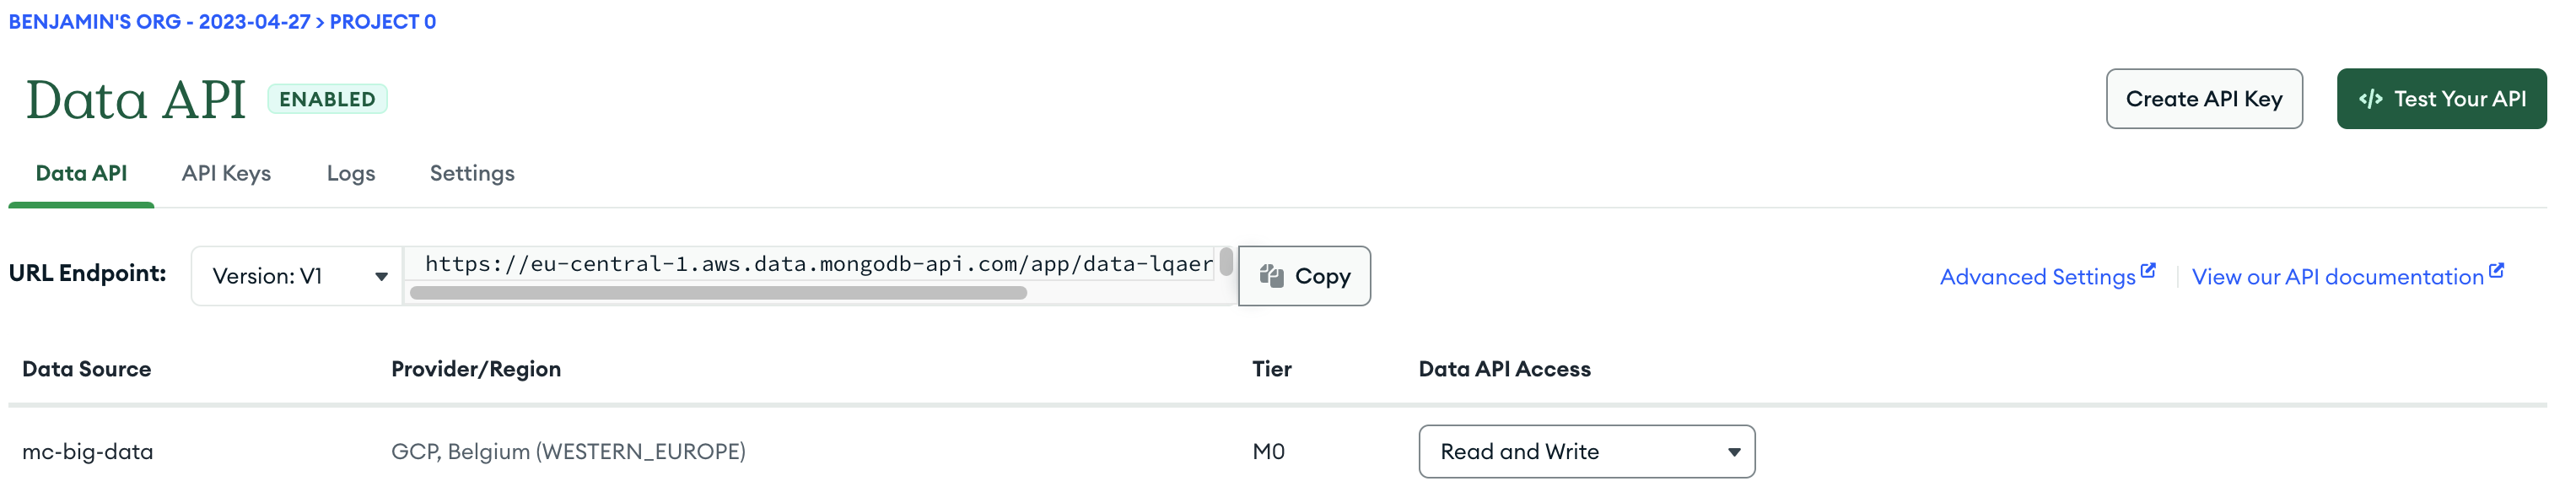
\includegraphics[width=\textwidth]{images/sc03.png}

	\vspace{0.5cm}
	\noindent \textcolor{red}{\textbf{Attention:}} The exercise steps tell us to create a new person Grandma Mary.
	Since Grandma Mary fits much better to the Folks than to the Persons I decided to make her a Folk.
	\vspace{0.2cm}

	\noindent \textbf{Create a new $\cancelto{Folk}{\textrm{Person}}$ - Grandma Mary:}
	\begin{lstlisting}[style=sql]
CREATE (grandma:Folk {name: "Grandma Mary"});
	\end{lstlisting}

	\noindent \textbf{Make Grandma Mary Mother of Mom and Dad:}
	\begin{lstlisting}[style=sql]
MATCH (mom:Folk {name: 'Mom'})
MATCH (dad:Folk {name: 'Dad'})
MATCH (grandma:Folk {name: 'Grandma Mary'})

CREATE (grandma)-[:MOTHER]->(mom)
CREATE (grandma)-[:MOTHER]->(dad);
	\end{lstlisting}

	\pagebreak

	\noindent \textbf{Return the ancestors of Alex as nodes:}
	\begin{lstlisting}[style=sql]
MATCH (alex:Folk {name: 'Alex'})
OPTIONAL MATCH path = (alex)<-[:MOTHER|FATHER*]-(ancestor:Folk)
RETURN DISTINCT ancestor AS ancestors;
	\end{lstlisting}
	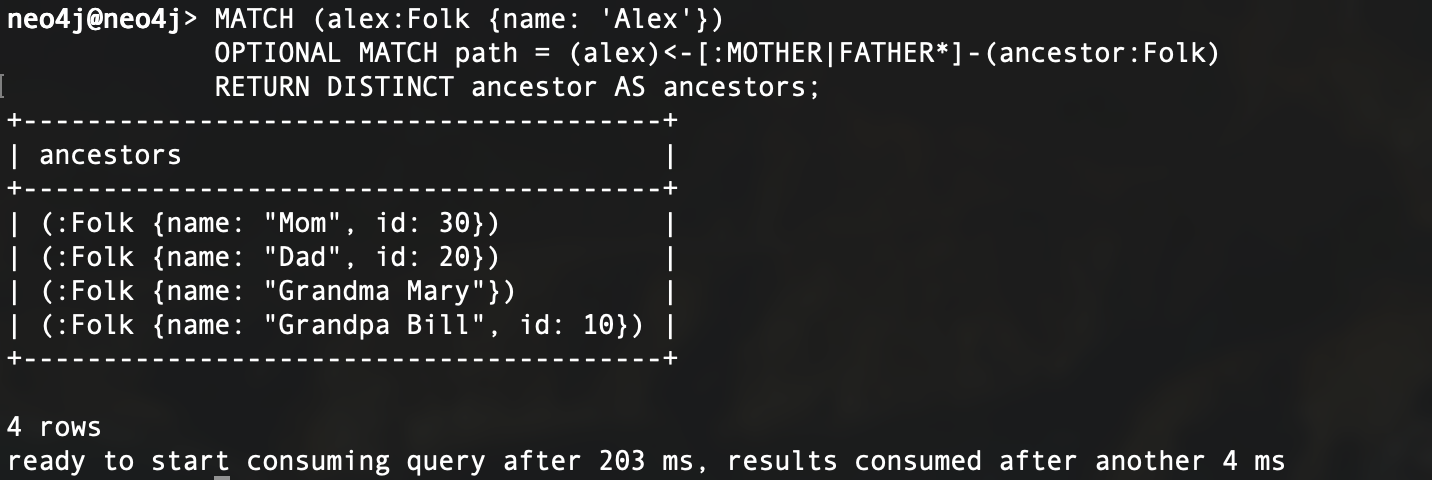
\includegraphics[width=\textwidth]{images/sc04.png}

	\noindent \textbf{Return the names of the ancestors of Alex:}
	\begin{lstlisting}[style=sql]
MATCH (alex:Folk {name: 'Alex'})
OPTIONAL MATCH path = (alex)<-[:MOTHER|FATHER*]-(ancestor:Folk)
RETURN DISTINCT ancestor.name AS ancestors;
	\end{lstlisting}
	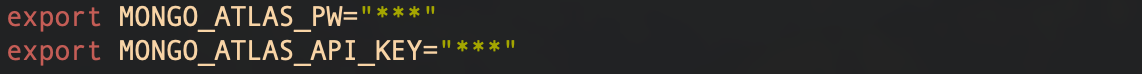
\includegraphics[width=\textwidth]{images/sc05.png}

	\noindent \textbf{Create Grandpa Jim and make him father of mom and dad:}
	\begin{lstlisting}[style=sql]
MATCH (mom:Folk {name: 'Mom'})
MATCH (dad:Folk {name: 'Dad'})

CREATE (grandpajim:Folk {name: 'Grandpa Jim'})

CREATE (grandpajim)-[:FATHER]->(mom)
CREATE (grandpajim)-[:FATHER]->(dad);
	\end{lstlisting}

	\pagebreak


	\noindent \textbf{Get the ancestor tree of Grandpa Jim:}
	\begin{lstlisting}[style=sql]
MATCH (grandpaJim:Folk {name: 'Grandpa Jim'})
MATCH path=(grandpaJim)-[*]->(ancestor)
RETURN DISTINCT ancestor as ancestortree, path;
	\end{lstlisting}
	\begin{center}
		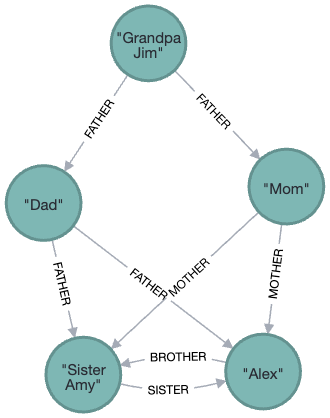
\includegraphics[height=5cm]{images/at_jim.png}
	\end{center}

	\noindent \textbf{Marry Mom with Dad and Grandma with Grandpa:}
	\begin{lstlisting}[style=sql]
MATCH (mom:Folk {name: 'Mom'})
MATCH (dad:Folk {name: 'Dad'})

MATCH (grandpaJim:Folk {name: 'Grandpa Jim'})
MATCH (grandmaMary:Folk {name: 'Grandma Mary'})

CREATE (mom)-[:MARRIED]->(dad)
CREATE (dad)-[:MARRIED]->(mom)

CREATE (grandpaJim)-[:MARRIED]->(grandmaMary)
CREATE (grandmaMary)-[:MARRIED]->(grandpaJim);
	\end{lstlisting}

	\noindent \textbf{Get the ancestor tree of Grandpa Jim without the married edges}
	\begin{lstlisting}[style=sql]
MATCH (grandpaJim:Folk {name: 'Grandpa Jim'})
MATCH path=(grandpaJim)-[*]->(ancestor)
WHERE NONE(rel IN relationships(path) WHERE type(rel) = 'MARRIED')
RETURN DISTINCT ancestor AS ancestortree, path;
	\end{lstlisting}
	\begin{center}
		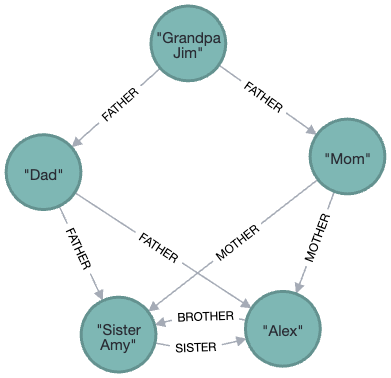
\includegraphics[height=5cm]{images/at_jim_2.png}
	\end{center}

	\pagebreak

	\subsection*{Add properties to nodes and eges}
	\noindent \textbf{Married properties:}
	\begin{lstlisting}[style=sql]
MATCH (mom:Folk {name: 'Mom'})
MATCH (dad:Folk {name: 'Dad'})

MATCH (grandpaJim:Folk {name: 'Grandpa Jim'})
MATCH (grandmaMary:Folk {name: 'Grandma Mary'})

MATCH (mom)-[momMarriedDad:MARRIED]->(dad)
MATCH (dad)-[dadMarriedMom:MARRIED]->(mom)
MATCH (grandpaJim)-[jimMarriedMary:MARRIED]->(grandmaMary)
MATCH (grandmaMary)-[maryMarriedJim]->(grandpaJim)

SET momMarriedDad.year = '2000'
SET dadMarriedMom.year = '2000'
SET jimMarriedMary.year = '1970'
SET maryMarriedJim.year = '1970';
	\end{lstlisting}

	\noindent \textbf{Born Year:}
	\begin{lstlisting}[style=sql]
MATCH (alex:Folk {name: 'Alex'})
MATCH (amy:Folk {name: 'Sister Amy'})

MATCH (mom:Folk {name: 'Mom'})
MATCH (dad:Folk {name: 'Dad'})

MATCH (grandpaJim:Folk {name: 'Grandpa Jim'})
MATCH (grandmaMary:Folk {name: 'Grandma Mary'})

SET alex.born_year = '2002'
SET amy.born_year = '2005'

SET mom.born_year = '1980'
SET dad.born_year = '1985'

SET grandpaJim.born_year = '1950'
SET grandmaMary.born_year = '1947';
	\end{lstlisting}

	\pagebreak

	\noindent \textbf{Ancestor tree of persons born in year:}
	\begin{lstlisting}[style=sql]
MATCH (person:Folk)
WHERE person.born_year = '2002'
MATCH path=(ancestor)-[*]->(person)
RETURN DISTINCT ancestor as ancestortree, path;
	\end{lstlisting}
	\begin{center}
	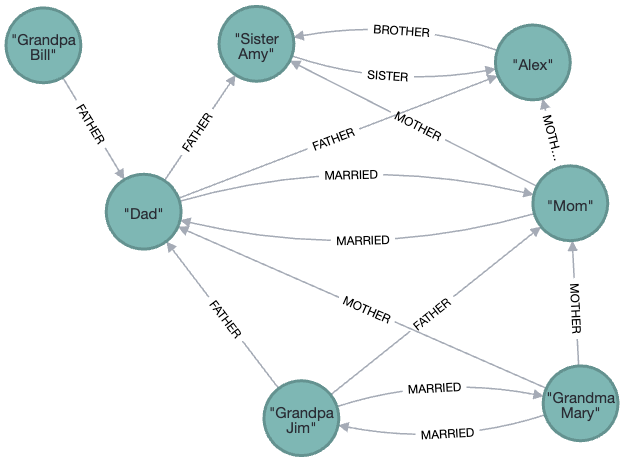
\includegraphics[height=5cm]{images/at_2002.png}
	\end{center}

	\noindent \textbf{Find Persons married in a particular year:}
	\begin{lstlisting}[style=sql]
MATCH (person:Folk)-[marriage:MARRIED]->(other:Folk)
WHERE marriage.year = '2000'
RETURN person, other;
	\end{lstlisting}

	%\noindent \textbf{Create API Key} \\
	%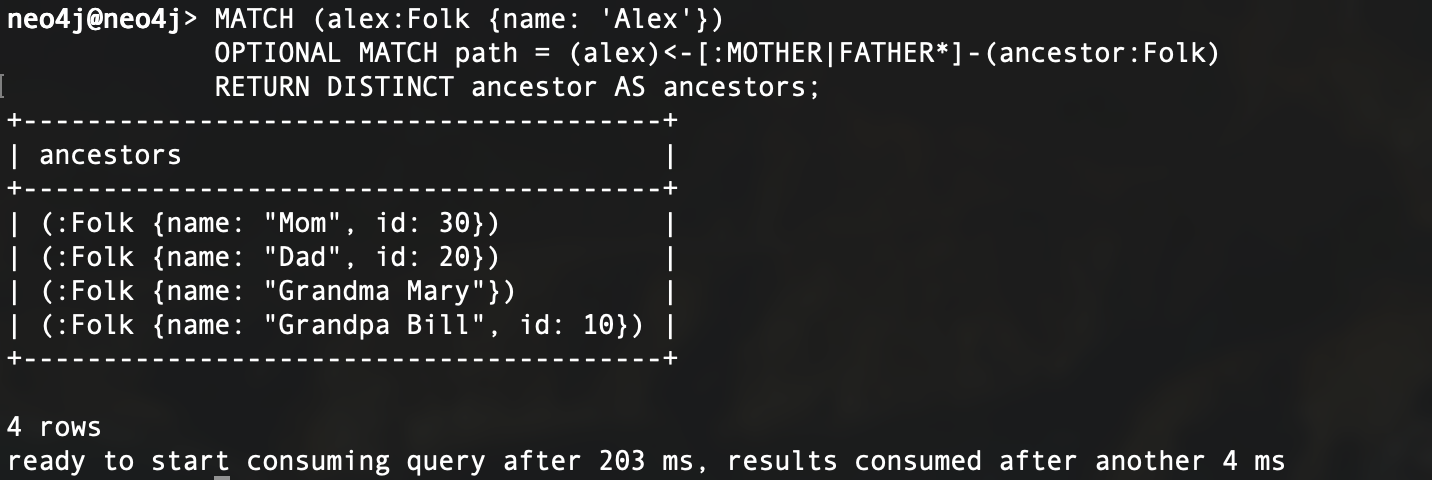
\includegraphics[width=\textwidth]{images/sc04.png}

	%\noindent \textbf{The pipeline fails because data is already in use} \\
	%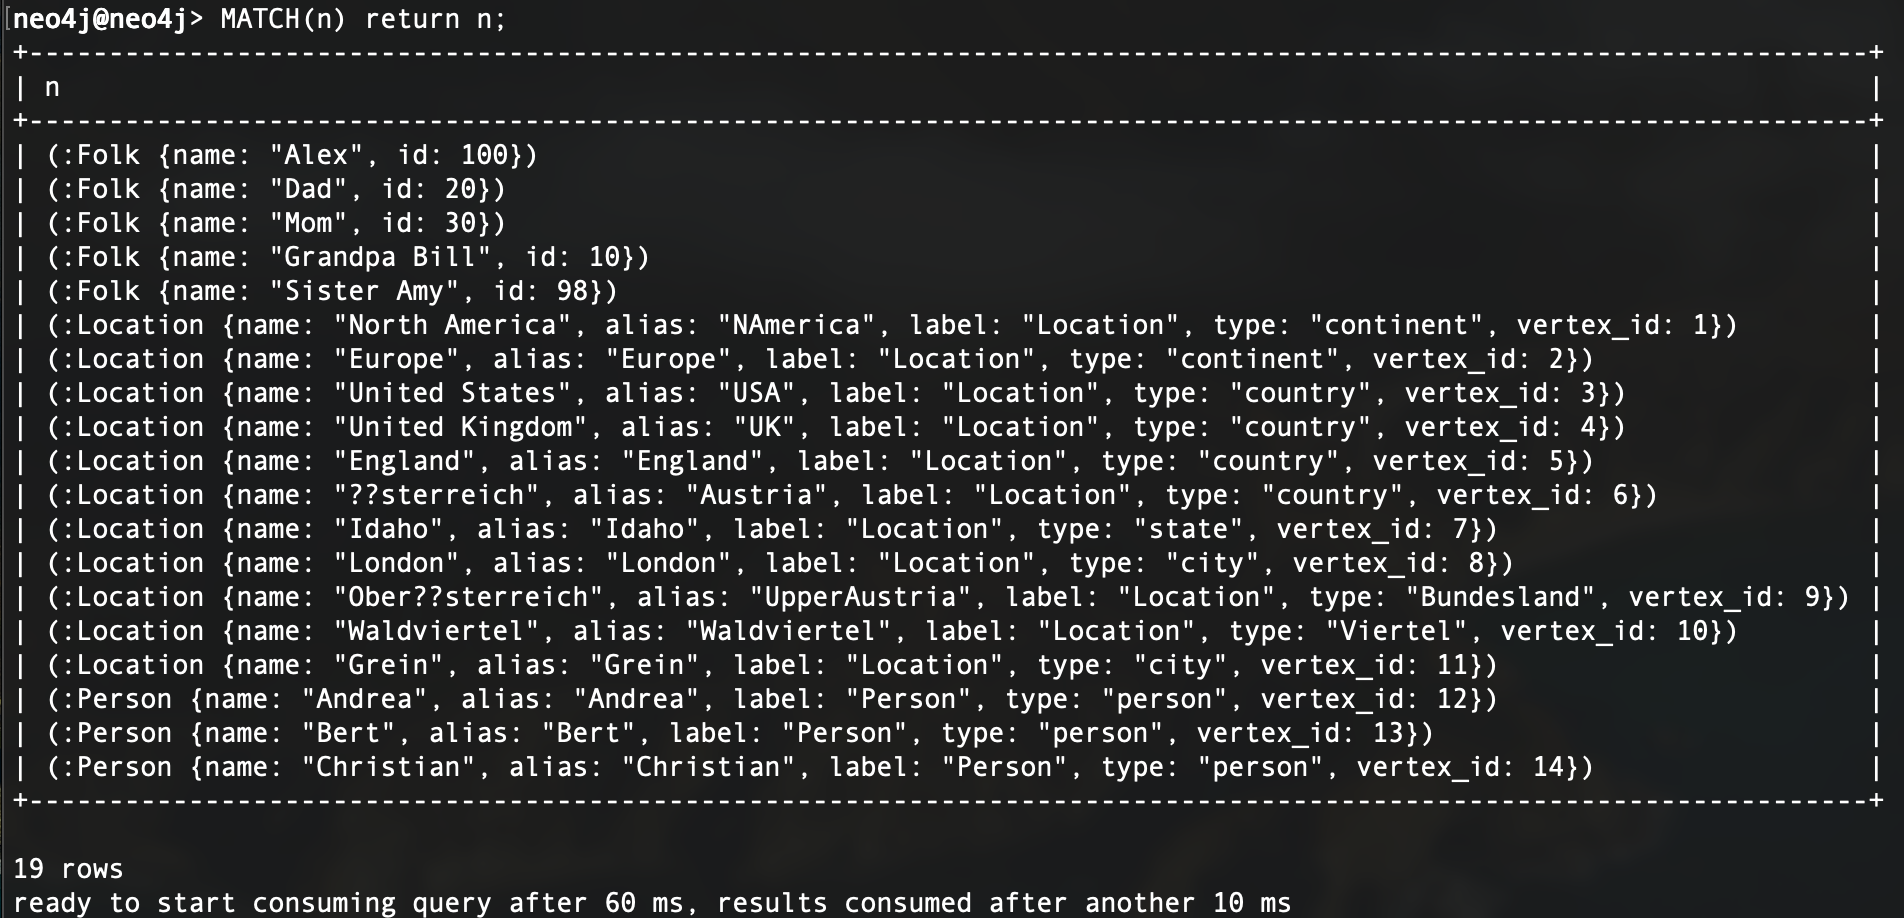
\includegraphics[width=\textwidth]{images/sc01.png} 
	%See \hyperref[listings:pipeline]{pipeline.conf} in appendix for the pipeline 
	%\begin{enumerate}[noitemsep]
		%\item Import the json file using mongoimport
	%\end{enumerate}

	%\newpage
	
	%\section*{Appendix}

	%\subsection*{.env}
	%\label{listings:envs}
	%\lstinputlisting[style=json]{.env}

	%\pagebreak

	\section*{Step 3:}
	\begin{lstlisting}[style=sql]
MATCH
(person)-[:BORN_IN]->()-[:WITHIN*0..]->(us:Location {name:'United States'}),
(person)-[:LIVES_IN]->()-[:WITHIN*0..]->(eu:Location {name:'Europe'})
WHERE person.label = 'Person'
RETURN person AS relevantPersons;
	\end{lstlisting}
	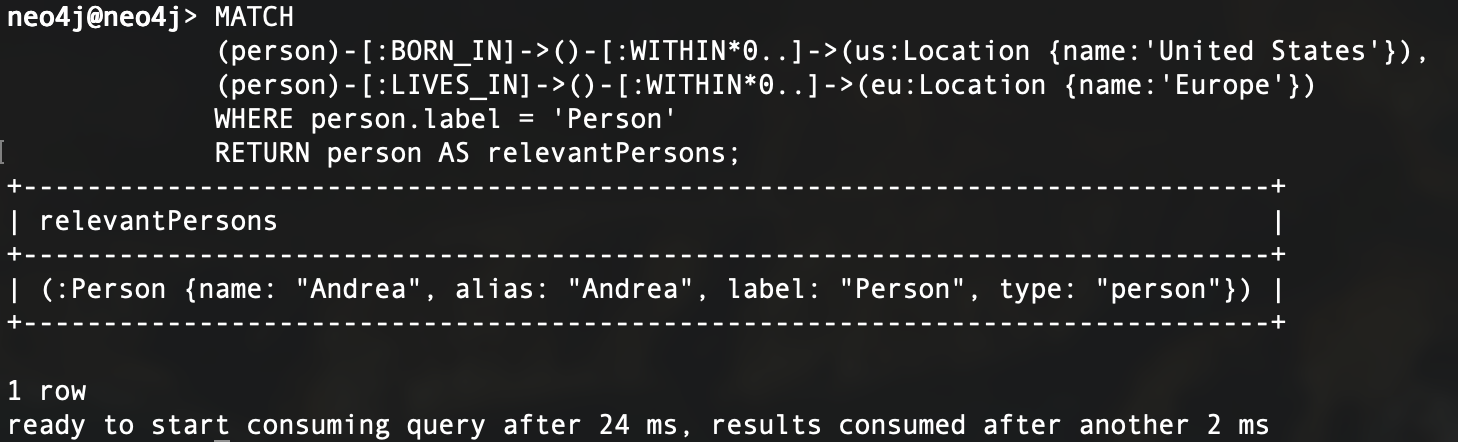
\includegraphics[width=\textwidth]{images/sc-step3.png}

	\newpage
	
	\section*{Step 4:}
	Since I am a cat fan, and because the names are funny I used the ancestor tree of my cat including the breeder and the new cat holder.

	\begin{lstlisting}[style=sql]
CREATE (lilly:Cat {name: 'Lilly', year_of_birth: '2022', gender: 'female'})
CREATE (lennox:Cat {name: 'Lennox', year_of_birth: '2022', gender: 'male'})
CREATE (lakota:Cat {name: 'Lakota', year_of_birth: '2022', gender: 'male'})

CREATE (nikanor:Cat {name: 'Nikanor Laminur', year_of_birth: '2020', gender: 'male'})
CREATE (fibi:Cat {name: 'Fibi Tandillo', year_of_birth: '2020', gender: 'female'})

CREATE (bc:Cat {name: 'Benjamin Chemchug', year_of_birth: '2016', gender: 'male'})
CREATE (dt:Cat {name: 'Dashutka Tale', year_of_birth: '2016', gender: 'female'})

CREATE (mk:Cat {name: 'Mozart Kocilandia', year_of_birth: '2014', gender: 'male'})
CREATE (nm:Cat {name: 'Naomi Mizar', year_of_birth: '2016', gender: 'female'})

CREATE (benjamin:Person {name: 'Benjamin'})
CREATE (iris:Person {name: 'Iris'})

CREATE (rpp:Breeder {name: 'Royal Pink Paws'})

CREATE (tieber:Family {name: 'Fam. Tieber'})
CREATE (wurm:Family {name: 'Fam. Wurm'})

CREATE (lilly)-[:SISTER]->(lennox)
CREATE (lilly)-[:SISTER]->(lakota)

CREATE (lennox)-[:BROTHER]->(lilly)
CREATE (lennox)-[:BROTHER]->(lakota)

CREATE (lakota)-[:BROTHER]->(lilly)
CREATE (lakota)-[:BROTHER]->(lennox)

CREATE (nikanor)-[:FATHER]->(lilly)
CREATE (nikanor)-[:FATHER]->(lennox)
CREATE (nikanor)-[:FATHER]->(lakota)

CREATE (fibi)-[:MOTHER]->(lilly)
CREATE (fibi)-[:MOTHER]->(lennox)
CREATE (fibi)-[:MOTHER]->(lakota)

CREATE (bc)-[:FATHER]->(nikanor)
CREATE (dt)-[:MOTHER]->(nikanor)

CREATE (mk)-[:FATHER]->(fibi)
CREATE (nm)-[:MOTHER]->(fibi)

CREATE (rpp)-[:BREEDER]->(lilly)
CREATE (rpp)-[:BREEDER]->(lennox)
CREATE (rpp)-[:BREEDER]->(lakota)

CREATE (benjamin)-[:BOYFRIEND]->(iris)
CREATE (iris)-[:GIRLFRIEND]->(benjamin)

CREATE (benjamin)-[:HOLDER]->(lilly)
CREATE (iris)-[:HOLDER]->(lilly)

CREATE (rpp)-[:HOLDER]->(nikanor)
CREATE (rpp)-[:HOLDER]->(fibi)

CREATE (tieber)-[:HOLDER]->(lennox)
CREATE (wurm)-[:HOLDER]->(lakota);
	\end{lstlisting}

	\begin{center}
		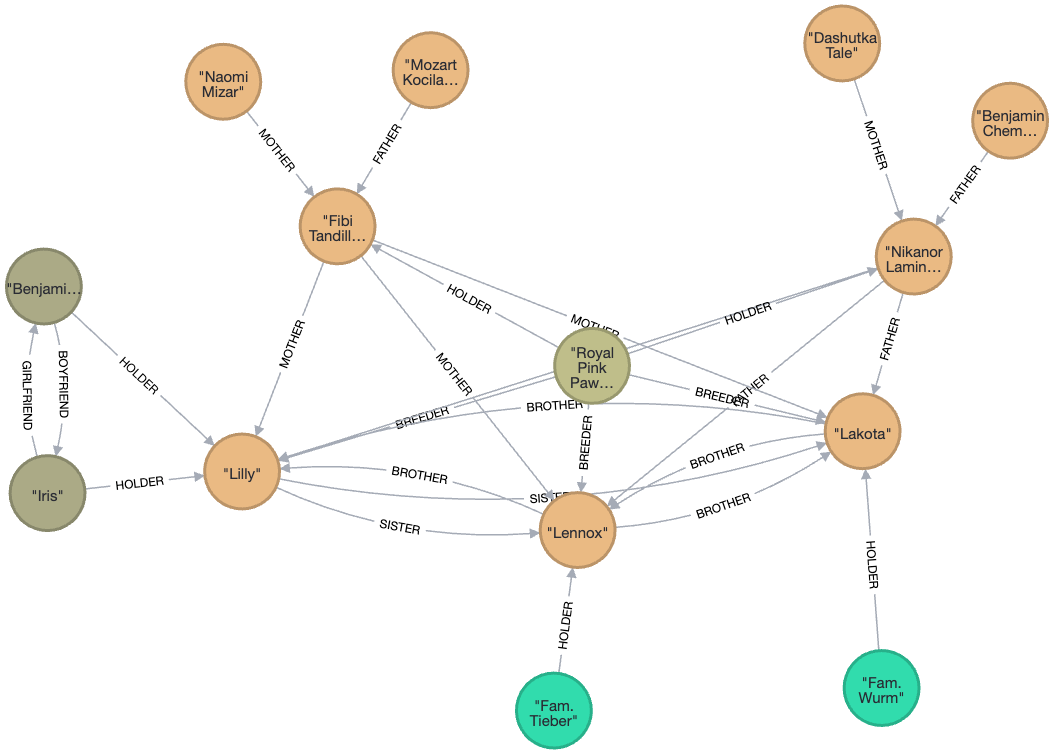
\includegraphics[width=0.8\textwidth]{images/cats.png}
	\end{center}
\end{document}
